\documentclass{article}

\usepackage{amsmath}
\usepackage{physics}
\usepackage{bbm}
\usepackage{listings}
\usepackage{verbatim}
\usepackage[utf8]{inputenc}
\usepackage{graphicx}

\title{Midterm ``Take home''-exam\\
		\large{FYS3110}}

\author{Candidate 83}

\date{\today}

\begin{document}

\maketitle

\section{Spin-$1/2$ systems}

The following is given:
\begin{align*}
\hat{S}^2 = \hat{S}_x^2+\hat{S}_y^2+\hat{S}_z^2, &\quad
\hat{S}^{\pm}=\hat{S}_x \pm i\hat{S}_y \\
\ket{\uparrow} \equiv \ket{s=\frac{1}{2},m_s=\frac{1}{2}}, &\quad 
\ket{\downarrow} \equiv \ket{s=\frac{1}{2},m_s=-\frac{1}{2}} \\
\hat{S}^2\ket{\uparrow} = \hbar^2\frac{1}{2}\left(\frac{1}{2}+1\right)\ket{\uparrow}, &\quad
\hat{S}^2\ket{\downarrow} = \hbar^2\frac{1}{2}\left(\frac{1}{2}+1\right)\ket{\downarrow} \\
\hat{S}_z\ket{\uparrow} = \frac{\hbar}{2}\ket{\uparrow}, &\quad 
\hat{S}_z\ket{\downarrow} = -\frac{\hbar}{2}\ket{\downarrow} \\
[\hat{S}_x,\hat{S}_y]=i\hbar\hat{S}_z, \quad
[\hat{S}_y,\hat{S}_z]&=i\hbar\hat{S}_x, \quad
[\hat{S}_z,\hat{S}_x]=i\hbar\hat{S}_y 
\end{align*}


%% -------------------- PROBLEM 1.1 ------------------ %%
\subsection{}
\begin{equation*}
\hat{S}_z\hat{S}^+\ket{\downarrow} = \hat{S}_z\hat{S}_x\ket{\downarrow} + i\hat{S}_z\hat{S}_y\ket{\downarrow}
\end{equation*}
rewriting commutation relations
\begin{align*}
[\hat{S}_z,\hat{S}_x]=\hat{S}_z\hat{S}_x - \hat{S}_x\hat{S}_z =i\hbar\hat{S}_y  &\rightarrow
\hat{S}_z\hat{S}_x = i\hbar\hat{S}_y + \hat{S}_x\hat{S}_z \\
[\hat{S}_y,\hat{S}_z]=\hat{S}_y\hat{S}_z - \hat{S}_z\hat{S}_y =i\hbar\hat{S}_x  &\rightarrow
\hat{S}_z\hat{S}_y = \hat{S}_y\hat{S}_z - i\hbar\hat{S}_x,
\end{align*}
gives
\begin{align*}
\hat{S}_z\hat{S}^+\ket{\downarrow} &=(i\hbar\hat{S}_y+\hat{S}_x\hat{S}_z+i\hat{S}_y\hat{S}_z+\hbar\hat{S}_x)\ket{\downarrow} \\
&= \left(i\hbar\hat{S}_y -\frac{\hbar}{2}\hat{S}_x -i\frac{\hbar}{2}\hat{S}_y + \hbar\hat{S}_x \right) \ket{\downarrow} \\
&=\left(\frac{\hbar}{2}\hat{S}_x + i\frac{\hbar}{2} \hat{S}_y\right)\ket{\downarrow} = \frac{\hbar}{2}\hat{S}^+\ket{\downarrow}.
\end{align*}
This means that $\hat{S}^+\ket{\downarrow}$ is an eigenstate of $\hat{S}_z$ with eigenvalue $\hbar/2$.


%% ------------------- PROBLEM 1.2 --------------------- %%
\subsection{}
\begin{align*}
\hat{S}^-\hat{S}^+ &=(\hat{S}_x-i\hat{S}_y)(\hat{S}_x+i\hat{S}_y) \\
&= \hat{S}_x^2+i\hat{S}_x\hat{S}_y-i\hat{S}_y\hat{S}_x+\hat{S}_y^2 \\
&= \hat{S}_x^2+\hat{S}_y^2+i[\hat{S}_x,\hat{S}_y] \\
&= \hat{S}^2-\hat{S}_z^2-\hbar\hat{S}_z
\end{align*}
This can be used to compute the norm of $\ket{\psi_1} = \hat{S}^+\ket{\downarrow}$ and $\ket{\psi_2} = \hat{S}^+\ket{\uparrow}$.
\begin{align*}
\braket{\psi_1} &= \bra{\downarrow}\hat{S}^-\hat{S}^+\ket{\downarrow} = \bra{\downarrow}(\hat{S}^2-\hat{S}_z^2-\hbar\hat{S}_z)\ket{\downarrow} \\
&= \bra{\downarrow}\hbar^2\frac{1}{2}\left(\frac{1}{2} +1 \right)\ket{\downarrow} -\bra{\downarrow}\frac{\hbar^2}{4} \ket{\downarrow} +\bra{\downarrow}\frac{2\hbar^2}{4} \ket{\downarrow} \\
&= \frac{3\hbar^2}{4} -\frac{\hbar^2}{4}+\frac{2\hbar}{4} = \hbar^2 
\end{align*}
which means that $\norm{\ket{\psi_1}} = \hbar$.
\begin{align*}
\braket{\psi_2} &= \bra{\uparrow}\hat{S}^-\hat{S}^+\ket{\uparrow} = \bra{\uparrow}(\hat{S}^2-\hat{S}_z^2-\hbar\hat{S}_z)\ket{\uparrow} \\
&= \bra{\uparrow}\hbar^2\frac{1}{2}\left(\frac{1}{2} +1 \right)\ket{\uparrow} -\bra{\uparrow}\frac{\hbar^2}{4} \ket{\uparrow} -\bra{\uparrow}\frac{2\hbar^2}{4} \ket{\uparrow} \\
&= \frac{3\hbar^2}{4} -\frac{\hbar^2}{4}-\frac{2\hbar^2}{4} = 0
\end{align*}
which means that $\norm{\ket{\psi_2}} = 0$.

%% ------------------ PROBLEM 1.3 --------------------- %%
\subsection{}
Phases are chosen so that the following relations hold
\begin{equation*}
\hat{S}^+\ket{\downarrow}=\hbar\ket{\uparrow}, \quad \hat{S}^-\ket{\uparrow}=\hbar\ket{\downarrow}.
\end{equation*}
From the the previous problem we also know that $\hat{S}^+\ket{\uparrow}=0$, and because $\bra{\psi}\hat{S}^+\hat{S}^-\ket{\psi}=\bra{\psi}\hat{S}^-\hat{S}^+\ket{\psi}=0$ then $\hat{S}^-\ket{\downarrow}=0$.

Introducing a new state
\begin{equation*}
\ket{\phi}=\frac{1}{\sqrt{2}}(\ket{\uparrow}+e^{i\theta}\ket{\downarrow})
\end{equation*}
where $\theta$ is a real number. We wish to compute the ``uncertainty'' product $\sigma_{sx}^2\sigma_{sy}^2$ where
\begin{align*}
\sigma_{sx}^2 &= \bra{\phi}(\hat{S}_x-\bra{\phi}\hat{S}_x\ket{\phi} )^2\ket{\phi}  \\
\sigma_{sy}^2 &= \bra{\phi}(\hat{S}_y-\bra{\phi}\hat{S}_y\ket{\phi} )^2\ket{\phi}.
\end{align*}
First we need to find expressions for $\hat{S}_x$ and $\hat{S}_y$
\begin{align}
\label{eq:Sx}
\hat{S}^++\hat{S}^- &= (\hat{S}_x + i\hat{S}_y) + (\hat{S}_x-i\hat{S}_y) = 2\hat{S}_x 
\rightarrow \hat{S}_x = \frac{1}{2}(\hat{S}^++\hat{S}^-)\\
\label{eq:Sy}
\hat{S}^+-\hat{S}^- &= (\hat{S}_x + i\hat{S}_y) - (\hat{S}_x-i\hat{S}_y) = 2i\hat{S}_y 
\rightarrow \hat{S}_y = \frac{1}{2i}(\hat{S}^+-\hat{S}^-)
\end{align}
It will also make things easier to calculate $\hat{S}_x\ket{\uparrow}$, $\hat{S}_x\ket{\downarrow}$, $\hat{S}_y\ket{\uparrow}$ and $\hat{S}_y\ket{\downarrow}$. These values can be found using equations \ref{eq:Sx} and \ref{eq:Sy}.
\begin{align*}
\hat{S}_x\ket{\uparrow}		= \frac{\hbar}{2}\ket{\downarrow}& \quad
\hat{S}^2_x\ket{\uparrow}	= \frac{\hbar^2}{4}\ket{\uparrow}\\
\hat{S}_x\ket{\downarrow}	= \frac{\hbar}{2}\ket{\uparrow}& \quad
\hat{S}^2_x\ket{\downarrow}	= \frac{\hbar^2}{4}\ket{\downarrow}\\
\hat{S}_y\ket{\uparrow}		= -\frac{\hbar}{2i}\ket{\downarrow}& \quad
\hat{S}^2_y\ket{\uparrow}	= \frac{\hbar^2}{4}\ket{\uparrow}\\
\hat{S}_y\ket{\downarrow}	= \frac{\hbar}{2i}\ket{\uparrow}& \quad
\hat{S}^2_y\ket{\downarrow}	= \frac{\hbar^2}{4}\ket{\downarrow}\\
\end{align*}
A few more pieces of the problem will be nice to have
\begin{align*}
\hat{S}^{+2}\ket{\phi}&=\hat{S}^{+2}(\ket{\uparrow}+e^{i\theta}\ket{\downarrow})=\hbar\hat{S}^{+}e^{i\theta}\ket{\uparrow}=0 \\
\hat{S}^{-2}\ket{\phi}&=\hat{S}^{-2}(\ket{\uparrow}+e^{i\theta}\ket{\downarrow})=\hbar\hat{S}^{-}\ket{\downarrow}=0 \\
\hat{S}^+\hat{S}^-\ket{\phi}&=\hat{S}^+\hat{S}^-\frac{1}{\sqrt{2}}(\ket{\uparrow}+e^{i\theta}\ket{\downarrow})=\frac{\hbar}{\sqrt{2}}\hat{S}^+\ket{\downarrow} = \frac{\hbar^2}{\sqrt{2}}\ket{\uparrow} \\
\hat{S}^-\hat{S}^+\ket{\phi}&=\hat{S}^-\hat{S}^+\frac{1}{\sqrt{2}}(\ket{\uparrow}+e^{i\theta}\ket{\downarrow})=\frac{\hbar}{\sqrt{2}}\hat{S}^-e^{i\theta}\ket{\uparrow} = \frac{\hbar^2}{\sqrt{2}}e^{i\theta}\ket{\downarrow}
\end{align*}
% Anticommutator
\begin{equation*}
\{\hat{S}^+,\hat{S}^-\}\ket{\phi}=(\hat{S}^+\hat{S}^-+\hat{S}^-\hat{S}^+)
\frac{1}{\sqrt{2}}(\ket{\uparrow}+e^{i\theta}\ket{\downarrow})=\frac{\hbar^2}{\sqrt{2}}(\ket{\uparrow}+e^{i\theta}\ket{\downarrow}) =\hbar^2\ket{\phi}
\end{equation*}
We can begin on what is the real task at hand
\begin{align*}
\bra{\phi}\hat{S}_x\ket{\phi} 
&= \frac{1}{2}(\bra{\uparrow}+e^{-i\theta}\bra{\downarrow})\hat{S}_x(\ket{\uparrow}+e^{i\theta}\ket{\downarrow}) \\
&= \frac{1}{2}(\bra{\uparrow}+e^{-i\theta}\bra{\downarrow})\left(\frac{\hbar}{2}\ket{\downarrow}+e^{i\theta}\frac{\hbar}{2}\ket{\uparrow} \right) \\
&= \frac{\hbar}{4}\left(e^{i\theta}+e^{-i\theta} \right)\\ 
&= \frac{\hbar}{4}(\cos{\theta}+i\sin{\theta}+\cos{\theta}-i\sin{\theta}) \\
&= \frac{\hbar}{2}\cos{\theta}
\end{align*}
\begin{align*}
\bra{\phi}\hat{S}_y\ket{\phi} 
&= \frac{1}{2}(\bra{\uparrow}+e^{-i\theta}\bra{\downarrow})\hat{S}_y(\ket{\uparrow}+e^{i\theta}\ket{\downarrow}) \\
&= \frac{1}{2}(\bra{\uparrow}+e^{-i\theta}\bra{\downarrow})\left(-\frac{\hbar}{2i}\ket{\downarrow}+e^{i\theta}\frac{\hbar}{2i}\ket{\uparrow} \right) \\
&= \frac{\hbar}{4i}\left(e^{i\theta}-e^{-i\theta} \right)\\ 
&= \frac{\hbar}{4i}(\cos{\theta}+i\sin{\theta}-\cos{\theta}+i\sin{\theta}) \\
&= \frac{\hbar}{2}\sin{\theta}
\end{align*}
Employing all of the above for the last algebraic exercise
\begin{equation}
\label{eq:sigmax}
\sigma_x^2=\bra{\phi}(\hat{S}^x-\bra{\phi}\hat{S}^x\ket{\phi})^2\ket{\phi} =
\bra{\phi}(\hat{S}^{x2}-\hbar\cos\theta\hat{S}^x+\frac{\hbar^2}{4}\cos^2\theta)\ket{\phi}
\end{equation}
where
\begin{align*}
\bra{\phi}\hat{S}^{x2}\ket{\phi} &= \frac{1}{4}\bra{\phi}(\hat{S}^+ + S^-)^2\ket{\phi}
=\frac{1}{4}\bra{\phi}(\hat{S}^++\{\hat{S}^+,\hat{S}^-\}+\hat{S}^-)\ket{\phi} = \frac{\hbar^2}{4}
\end{align*}
and
\begin{equation*}
\bra{\phi}\hbar\cos\theta\hat{S}^x\ket{\phi} = \frac{2}{4}\hbar^2\cos^2\theta
\end{equation*}
Equation \ref{eq:sigmax} becomes
\begin{equation}
\sigma_x^2=\frac{\hbar^2}{4}-\frac{2\hbar}{4}\cos\theta+\frac{\hbar^2}{4}\cos^2\theta =
\frac{\hbar^2}{4}(1-\cos^2\theta)=\frac{\hbar^2}{4}\sin^2\theta
\end{equation}
Now for the other part of the product
\begin{equation}
\label{eq:sigmay}
\sigma_y^2=\bra{\phi}(\hat{S}^y-\bra{\phi}\hat{S}^y\ket{\phi})^2\ket{\phi} =
\bra{\phi}(\hat{S}^{y2}-\hbar\sin\theta\hat{S}^y+\frac{\hbar^2}{4}\sin^2\theta)\ket{\phi}
\end{equation}
where
\begin{align*}
\bra{\phi}\hat{S}^{y2}\ket{\phi} &= -\frac{1}{4}\bra{\phi}(\hat{S}^+ - S^-)^2\ket{\phi}
=-\frac{1}{4}\bra{\phi}(\hat{S}^+-\{\hat{S}^+,\hat{S}^-\}+\hat{S}^-)\ket{\phi} = \frac{\hbar^2}{4}
\end{align*}
and
\begin{equation*}
\bra{\phi}\hbar\sin\theta\hat{S}^y\ket{\phi} = \frac{2}{4}\hbar^2\sin^2\theta
\end{equation*}3
Equation \ref{eq:sigmay} becomes
\begin{equation}
\sigma_y^2 = \frac{\hbar^2}{4}-\frac{2\hbar^2}{4}\sin^2\theta+\frac{\hbar^2}{4}\sin^2\theta =
\frac{\hbar^2}{4}(1-\sin^2\theta)=\frac{\hbar^2}{4}\cos^2\theta
\end{equation}
The product of equation \ref{eq:sigmax} and equation \ref{eq:sigmay} is
\begin{equation}
\label{eq:heisenbergish}
\sigma_x^2\sigma_y^2=\frac{\hbar^4}{16}(\sin^2\theta\cos^2\theta)=\frac{\hbar^4}{32}\sin^2{(2\theta)}
\end{equation}
which is zero for $\theta=0$ and $\theta=\pi/2$. Does this violate Heisenberg's uncerainty principle? Not necessarily.

The generalized Heisenberg uncertainty is given by 
\begin{equation}
\label{eq:heisenberg}
\sigma_x\sigma_y \geq \frac{1}{2}\abs{\ev{[\hat{S}_x,\hat{S}_y]}}=\frac{1}{2}\abs{i\hbar\ev{\hat{S}_z}}
\end{equation}
Computing the expected value of the spin-operator along the $z$-axis
\begin{align*}
\ev{\hat{S}_z}&=\bra{\phi}\hat{S}_z\ket{\phi} = \frac{1}{2}(\bra{\uparrow}+e^{-i\theta}\bra{\downarrow})\hat{S}_z(\ket{\uparrow}+e^{i\theta}\ket{\downarrow} \\
&= \frac{\hbar}{4}(\bra{\uparrow} + e^{-i\theta}\bra{\downarrow})(\ket{\uparrow}-e^{i\theta}\ket{\downarrow}) = \frac{\hbar}{4}(1-1)=0
\end{align*}
interting this into equation \ref{eq:heisenberg} yields 0. We see that Heisenberg's uncertainty principle is not violated, because 
\begin{equation}
\sigma_x\sigma_y \geq 0
\end{equation}

Furthermore, only one of the components of the product in equation \ref{eq:heisenbergish} is zero, $\sigma_x^2=0$ while $\sigma_y^2=\hbar^2/4$.
\begin{equation}
\phi=
\begin{cases}
\frac{1}{\sqrt{2}}(\ket{\uparrow} + \ket{\downarrow}), &\text{for } \theta = 0, \\
\frac{1}{\sqrt{2}}(\ket{\uparrow} + i\ket{\downarrow}), &\text{for } \theta = \frac{\pi}{2}
\end{cases}
\end{equation}


%% -------------- PROBLEM 1.4 ---------------- %%
\subsection{}
A system has three interacting spin degrees of freedom with the followin hamiltonian
\begin{equation}
H = \frac{J}{\hbar^2}(\vb{S}_1\cdot\vb{S}_2 + \vb{S}_2\cdot\vb{S}_3 + \vb{S}_3\cdot\vb{S}_1)
\end{equation}
where $J$ is a positive number with units of energy. The spin operators are $\vb{S}_1\equiv \vb{S}\otimes\mathbbm{1}\otimes\mathbbm{1}$, $\vb{S}_2\equiv \mathbbm{1}\otimes\vb{S}\otimes\mathbbm{1}$ and $\vb{S}_3\equiv \mathbbm{1}\otimes\mathbbm{1}\otimes\vb{S}$, where $\vb{S}=(S_x,S_y,S_z)$. A general state of this three-spin system is a linear combination of product states $\ket{m_{s1}m_{s2}m_{s3}}\equiv\ket{m_{s1}}\otimes\ket{m_{s2}}\otimes\ket{m_{s3}}$ where $m_{si}$ is the spin-$z$ quantum number of spin number $i$, either up ($\frac{1}{2}$) or down ($-\frac{1}{2}$). For example: the product state $\ket{\uparrow\downarrow\uparrow}$ is a state where spin number one is in state $\ket{\uparrow}$, spin number two is in state $\ket{\downarrow}$ and spin number three is in state $\ket{\uparrow}$.

$\vb{S}_1\cdot\vb{S}_2$ can be expressed in terms of $S_1^+$, $S_1^-$, $S_2^+$, $S_2^-$, $S_1^z$ and $S_2^z$. First we have
\begin{equation*}
\vb{S}_1\cdot\vb{S}_2=S_1^xS_2^x + S_1^yS_2^y + S_1^zS_2^z
\end{equation*}
where
\begin{align*}
S_1^xS_2^x= \frac{1}{4}(S_1^+S_2^+ +S_1^+S_2^- + S_1^-S_2^+ + S_1^+S_2^-)\\
S_1^yS_2^y=-\frac{1}{4}(S_1^+S_2^+ -S_1^+S_2^- - S_1^-S_2^+ + S_1^+S_2^-)
\end{align*}
\begin{comment}then
\begin{equation*}
S_1^xS_2^x + S_1^yS_2^y = S_1^+S_2^-
\end{equation*}
assuming that the lowering and raising operators of different spins commute\footnote{Ladder operator for same spin/state commute: $[S^+,S^-]=(S^x+iS^y)(S^x-iS^y)-(S^x-iS^y)(S^x+iS^y)=S_x^2+S_y^2-S_x^2-S_y^2$=0}, i.e. $[S_i^+,S_j^-]=0$. We end up with
\begin{equation}
\vb{S}_1\cdot\vb{S}_2 = S_1^+S_2^- + S_1^zS_2^z
\end{equation}
\end{comment}
If the ladder operators does not commute then
\begin{equation*}
S_1^xS_2^x + S_1^yS_2^y = \frac{1}{2}(S_1^+S_2^- + S_2^+S_1^-)
\end{equation*}
and we end up with
\begin{equation}
\vb{S}_1\cdot\vb{S}_2 = \frac{1}{2}(S_1^+S_2^- + S_2^+S_1^-) + S_1^zS_2^z
\end{equation}

Computing $H\ket{\uparrow\downarrow\downarrow}$ should now be quite straight-forward.
\begin{align*}
H\ket{\uparrow\downarrow\downarrow} = 
\frac{J}{\hbar^2} \big(&\frac{1}{2} (S_1^+S_2^- + S_2^+S_1^-)\ket{\uparrow\downarrow\downarrow} + S_1^zS_2^z\ket{\uparrow\downarrow\downarrow} \\
+&\frac{1}{2}(S_2^+S_3^- + S_3^+S_2^-)\ket{\uparrow\downarrow\downarrow} + S_2^zS_3^z\ket{\uparrow\downarrow\downarrow} \\
+&\frac{1}{2}(S_3^+S_1^- + S_1^+S_3^-)\ket{\uparrow\downarrow\downarrow} + S_3^zS_1^z\ket{\uparrow\downarrow\downarrow} \big)\\
=&\frac{J}{\hbar^2}\big(
\frac{\hbar^2}{2}\ket{\downarrow\uparrow\downarrow} + 
\frac{\hbar^2}{2}\ket{\downarrow\downarrow\uparrow} -
\frac{\hbar^2}{4}\ket{\uparrow\downarrow\downarrow} 
\big) \\
=&J(
\frac{1}{2}\ket{\downarrow\uparrow\downarrow} +
\frac{1}{2}\ket{\downarrow\downarrow\uparrow} -
\frac{1}{4}\ket{\uparrow\downarrow\downarrow})
\end{align*}

This result is confirmed by the python script in appendix \ref{app:updndn}. One can conclude that $\ket{\uparrow\downarrow\downarrow}$ is not an eigenstate of $H$.

%% --------------- PROBLEM 1.5 -------------- %%
\subsection{}
It is realtively easy, yet tiresome, to show (with matrices or algebra or a script or anything) that
\begin{equation}
[H,S^z_{tot}]=0.
\end{equation}
Most of the terms will cancel each other out, but one will also need the following commutating relations
\begin{align*}
[S^+,S^z]&=S^+S^z-S^zS^+ = S^xS^z+iS^yS^z-S^zS^x-iS^zS^y \\
&= [S^x,S^z] + i[S^y, S^z] = -i\hbar S^y-\hbar S^x\\
[S^-,S^z]&=S^-S^z-S^zS^- = S^xS^z-iS^yS^z-S^zS^x+iS^zS^y \\
&= [S^x,S^z] + i[S^z, S^y] = -i\hbar S^y+\hbar S^x
\end{align*}
The rest of the calculation is in appendix \ref{app:prob1.5}\footnote{I have chosen not to include it because it woudld a nightmare to code in \LaTeX. I get the same result when doing the calculation with Pauli matrices in Python using the data structures in appendix \ref{app:updndn}}.

The eigenvalues of $S^z_{tot}$ are easy enough to compute
\begin{equation*}
S^z_{tot}\ket{\uparrow\uparrow\uparrow}=\frac{\hbar}{2}\ket{\uparrow\uparrow\uparrow}+\frac{\hbar}{2}\ket{\uparrow\uparrow\uparrow} + \frac{\hbar}{2}\ket{\uparrow\uparrow\uparrow} = \frac{3\hbar}{2}\ket{\uparrow\uparrow\uparrow}
\end{equation*}
the rest are
\begin{align*}
S^z_{tot}\ket{\uparrow\uparrow\downarrow}&=\frac{\hbar}{2}\ket{\uparrow\uparrow\downarrow} \\
S^z_{tot}\ket{\uparrow\downarrow\uparrow}&=\frac{\hbar}{2}\ket{\uparrow\downarrow\uparrow} \\
S^z_{tot}\ket{\downarrow\uparrow\downarrow}&=\frac{\hbar}{2}\ket{\downarrow\uparrow\downarrow} \\
S^z_{tot}\ket{\downarrow\downarrow\uparrow}&=-\frac{\hbar}{2}\ket{\downarrow\downarrow\uparrow} \\
S^z_{tot}\ket{\downarrow\uparrow\downarrow}&=-\frac{\hbar}{2}\ket{\downarrow\uparrow\downarrow} \\
S^z_{tot}\ket{\uparrow\downarrow\downarrow}&=-\frac{\hbar}{2}\ket{\uparrow\downarrow\downarrow} \\
S^z_{tot}\ket{\downarrow\downarrow\downarrow}&=-\frac{3\hbar}{2}\ket{\downarrow\downarrow\downarrow} 
\end{align*}

The ``general'' rule appears to be
\begin{equation}
S^z_{tot}\ket{m_{s1}m_{s2}m_{s3}}=\hbar (m_{s1}+m_{s2}+m_{s3})\ket{m_{s1}m_{s2}m_{s3}}
\end{equation}


%% --------------- PROBLEM 1.6 -------------- %%
\subsection{}
Finding eigenvalues of $H$. The trick is first to express $H$ in terms of $S_{tot}^2$.
\begin{align*}
S_{tot}^2 &= S_1^2 + S_2^2 + S_3^2 + 2S_1\cdot S_2 + 2S_2\cdot S_3 + 2S_3\cdot S_1 \\
H &= \frac{J}{2\hbar^2}(2S_1\cdot S_2 + 2S_2\cdot S_3 + 2S_3\cdot S_1) \\
  &= \frac{J}{2\hbar^2}(S_{tot}^2-(S_1^2+S_2^2+S_3^3))
\end{align*}

We know from the previous problem that total spin angular momentum quantum number $s_{tot}$ must be $3/2$ or $1/2$. The general formula for the energy eigenvalue of total spin quantum number squared is $S^2_{tot}\ket{\psi}=s_{tot}(1+s_{tot})\hbar^2\ket{\psi}$. The eigenvalue energy for $s_{tot}=3/2$ is therefore given by
\begin{align*}
H\ket{\psi} =& \frac{J}{2\hbar^2}(S_{tot}^2\ket{\psi}-(S_1^2+S_2^2+S_3^2)\ket{\psi})\\
=&\frac{J}{2\hbar^2}\left(\frac{3}{2}\left(\frac{3}{2}+1\right)\hbar^2 +3\frac{1}{2}\left(\frac{1}{2}+1\right)\hbar^2\right)\ket{\psi}\\
=&\frac{J}{2\hbar^2}\left(\frac{15\hbar^2}{4}\ket{\psi} -3\frac{3\hbar^2}{4}\ket{\psi} \right) = J\frac{3}{4}\ket{\psi},
\end{align*}
and for $s_{tot}=1/2$
\begin{align*}
H\ket{\psi} =& \frac{J}{2\hbar^2}(S_{tot}^2\ket{\psi}-(S_1^2+S_2^2+S_3^2)\ket{\psi})\\
=&\frac{J}{2\hbar^2}\left(\frac{1}{2}\left(\frac{1}{2}+1\right)\hbar^2 +3\frac{1}{2}\left(\frac{1}{2}+1\right)\hbar^2\right)\ket{\psi}\\
=&\frac{J}{2\hbar^2}\left(\frac{3\hbar^2}{4}\ket{\psi} -3\frac{3\hbar^2}{4}\ket{\psi} \right) = -J\frac{3}{4}\ket{\psi}.
\end{align*}
The eigenvalues of $H$ is $\pm\frac{3}{4}J$.

%% --------------- PROBLEM 1.7 -------------- %%
\subsection{}
In order to write down the normalized eigenstates of $S_{tot}$ of total spin angular momentum quantum number $s_{tot}=\frac{1}{2}$ one must employ Clebsch-Gordan coefficient tables. First, combine two of the spins, and then the result with the third spin.
\begin{equation*}
\ket{s_1m_{s1}s_2m_{s2}s_3m_{s3}}=\ket{s_1m_{s1}s_2m_{s2}}\otimes\ket{s_3m_{s3}}=\ket{s_1m_{s1}}\otimes\ket{s_2m_{s2}}\otimes\ket{s_3m_{s3}}
\end{equation*}

A system of two spin-$1/2$ particles can have $s_{tot}=0$ and $s_{tot}=1$. The former case, the singlet, has only one possible linear combination of $s=1/2$ kets
\begin{equation}
\label{eq:spins0}
\ket{0,0}=\frac{1}{\sqrt{2}}\ket{\frac{1}{2},+\frac{1}{2}}\otimes\ket{\frac{1}{2},-\frac{1}{2}}-\frac{1}{\sqrt{2}}\ket{\frac{1}{2},-\frac{1}{2}}\otimes\ket{\frac{1}{2},+\frac{1}{2}},
\end{equation}
while if $s=1$ we have the triplet
\begin{align}
\label{eq:spins1-1}
&\ket{1,-1} = \ket{\frac{1}{2},\frac{1}{2}}\otimes\ket{\frac{1}{2},-\frac{1}{2}} \\
\label{eq:spins10}
&\ket{1, 0} = \frac{1}{\sqrt{2}}\ket{\frac{1}{2},+\frac{1}{2}}\otimes\ket{\frac{1}{2},-\frac{1}{2}} + \frac{1}{\sqrt{2}}\ket{\frac{1}{2},-\frac{1}{2}}\otimes\ket{\frac{1}{2},+\frac{1}{2}} \\
\label{eq:spins1+1}
&\ket{1,+1} = \ket{\frac{1}{2},+\frac{1}{2}}\otimes\ket{\frac{1}{2},+\frac{1}{2}}
\end{align}

Combining the combined spins where $s=0$ with a third spin is relatively simple. The tensor product of an $s=0$ particle with another particle is simply the latter particle. One needs to combine the singlet in equation \ref{eq:spins0} with $\ket{\uparrow}$ and $\ket{\downarrow}$
\begin{align*}
&\ket{0,0}\otimes\ket{\frac{1}{2},+\frac{1}{2}} \\
&=\frac{1}{\sqrt{2}}\ket{\frac{1}{2},+\frac{1}{2}}\otimes\ket{\frac{1}{2},-\frac{1}{2}}\otimes\ket{\frac{1}{2},+\frac{1}{2}}-\frac{1}{\sqrt{2}}\ket{\frac{1}{2},-\frac{1}{2}}\otimes\ket{\frac{1}{2},+\frac{1}{2}}\otimes\ket{\frac{1}{2},+\frac{1}{2}} \\
&\ket{0,0}\otimes\ket{\frac{1}{2},-\frac{1}{2}}= \\
&=\frac{1}{\sqrt{2}}\ket{\frac{1}{2},+\frac{1}{2}}\otimes\ket{\frac{1}{2},-\frac{1}{2}}\otimes\ket{\frac{1}{2},-\frac{1}{2}}-\frac{1}{\sqrt{2}}\ket{\frac{1}{2},-\frac{1}{2}}\otimes\ket{\frac{1}{2},+\frac{1}{2}}\otimes\ket{\frac{1}{2},-\frac{1}{2}}
\end{align*}
alternatively, in a simplified ``arrow notation''
\begin{align}
\frac{1}{\sqrt{2}}\ket{\uparrow\downarrow\uparrow}-\frac{1}{\sqrt{2}}\ket{\downarrow\uparrow\uparrow} \\
\frac{1}{\sqrt{2}}\ket{\uparrow\downarrow\downarrow}-\frac{1}{\sqrt{2}}\ket{\downarrow\uparrow\downarrow}
\end{align}

For the triplet, in equations \ref{eq:spins1-1}, \ref{eq:spins10} and \ref{eq:spins1+1} one must apply Clebsch-Gordan tables again. We want to combine the new spin-$1$ particles in equations \ref{eq:spins1-1}, \ref{eq:spins10} and \ref{eq:spins1+1} with another spin-$1/2$ particle. This can be found in the $1\times1/2$ table. We are only interested in the cases that have total spin $s_{tot}=1/2$ which leaves us with
\begin{align}
\label{eq:1timeshalf1}
\ket{\frac{1}{2},+\frac{1}{2}} &= \sqrt{\frac{2}{3}}\ket{1,+1}\otimes\ket{\frac{1}{2},-\frac{1}{2}}-\frac{1}{\sqrt{3}}\ket{1,0}\otimes\ket{\frac{1}{2},+\frac{1}{2}} \\
\label{eq:1timeshalf2}
\ket{\frac{1}{2},-\frac{1}{2}} &= \frac{2}{\sqrt{3}}\ket{1,0}\otimes\ket{\frac{1}{2},-\frac{1}{2}}-\sqrt{\frac{0}{3}}\ket{1,-1}\otimes\ket{\frac{1}{2},+\frac{1}{2}}
\end{align}
Inserting equations \ref{eq:spins1-1}, \ref{eq:spins10} and \ref{eq:spins1+1} into equations \ref{eq:1timeshalf1} and \ref{eq:1timeshalf2} yields
\begin{align*}
&\sqrt{\frac{2}{3}}\ket{\frac{1}{2},+\frac{1}{2}}\otimes\ket{\frac{1}{2},+\frac{1}{2}}\otimes\ket{\frac{1}{2},-\frac{1}{2}} \\
-&\frac{1}{\sqrt{6}}\ket{\frac{1}{2},+\frac{1}{2}}\otimes\ket{\frac{1}{2},-\frac{1}{2}}\otimes\ket{\frac{1}{2},+\frac{1}{2}} \\
-&\frac{1}{\sqrt{6}}\ket{\frac{1}{2},-\frac{1}{2}}\otimes\ket{\frac{1}{2},+\frac{1}{2}}\otimes\ket{\frac{1}{2},+\frac{1}{2}}, \\[3ex]
&\frac{1}{\sqrt{6}}\ket{\frac{1}{2},+\frac{1}{2}}\otimes\ket{\frac{1}{2},-\frac{1}{2}}\otimes\ket{\frac{1}{2},-\frac{1}{2}} \\
+&\frac{1}{\sqrt{6}}\ket{\frac{1}{2},-\frac{1}{2}}\otimes\ket{\frac{1}{2},+\frac{1}{2}}\otimes\ket{\frac{1}{2},-\frac{1}{2}} \\
-&\sqrt{\frac{2}{3}}\ket{\frac{1}{2},-\frac{1}{2}}\otimes\ket{\frac{1}{2},-\frac{1}{2}}\otimes\ket{\frac{1}{2},+\frac{1}{2}},
\end{align*}
or in ``arrow notation'' again
\begin{align}
\sqrt{\frac{2}{3}}\ket{\uparrow\uparrow\downarrow}-\frac{1}{\sqrt{6}}\ket{\uparrow\downarrow\uparrow}-\frac{1}{\sqrt{6}}\ket{\downarrow\uparrow\uparrow} \\
\frac{1}{\sqrt{6}}\ket{\uparrow\downarrow\downarrow}+\frac{1}{\sqrt{6}}\ket{\uparrow\downarrow\downarrow}-\sqrt{\frac{2}{3}}\ket{\downarrow\downarrow\uparrow}
\end{align}


%% --------------- PROBLEM 1.8 -------------- %%
\subsection{}
At time $t=0$ the system is in state $\ket{\uparrow\downarrow\downarrow}$. After som time $t$ the system will be in state $\hat{U}(t,t_0)\ket{\uparrow\downarrow\downarrow}$, where $\hat{U}(t,t_0)$ is the time evolution operator (or propagator). The propagator satisfy three important properties. First, it does nothing when $t=0$
\begin{equation}
\lim_{t\to t_0}\hat{U}(t,t0)=1.
\end{equation}
Second, it is unitary ($\hat{U}^{\dagger}\hat{U}=1$), and as a consequence preserves the norm of the states
\begin{equation}
\braket{\psi} = \braket{\psi(t)} = \bra{\psi(t)} \hat{U}^{\dagger}(t,t_0){U}(t,t_0) \ket{\psi(t)}
\end{equation}
Third, it satisfies the composition property
\begin{equation}
\hat{U}(t_2,t_0)=\hat{U}(t_2,t_1)\hat{U}(t_1,t_0)
\end{equation}

One can see from the simplest form of Scrhödinger's equation that the Hamiltonian $H$ generates the time evolution of quantum states. if $\ket{\psi(t)}$ is the state of the system at time $t$, then
\begin{equation}
H\ket{\psi(t)}=i\hbar\frac{\partial}{\partial t}\ket{\psi(t)}.
\end{equation}

Given the state at some initial time ($t=0$) one can solve Schrödinger's equation in order to obtain the state at any subsequent time. Particularly, if $H$ is independent of time, then
\begin{equation}
\ket{\psi(t)}=e^{-iHt/\hbar}\ket{\psi(0)} = e^{-iE_nt/\hbar}\ket{\psi(0)}.
\end{equation}
This exponential operator is usually defined by the corresponding power series. 
\begin{equation}
U(t) = \sum_{k=0}^{\infty}\frac{1}{k!}\left(\frac{it}{\hbar} \right)H^k = e^{-iHt/\hbar}
\end{equation}

If a spin system is initially in state $\ket{\uparrow\downarrow\downarrow}$ at $t_0=0$ then the real part of $\abs{\bra{\uparrow\downarrow\downarrow}\hat{U}(t,0) \ket{\uparrow\downarrow\downarrow}}^2$ gives the probability that the system is still in that state.

I have chosen to compute these probabilities using a numerical approach. The components of the Hamiltonian can all be represented by Pauli matrices. These are the same matrices that are calculated in appendix \ref{app:updndn}. In the following computation, both $J$ and $\hbar$ is set to $1$, which is perfectly alright as the solution will be the same. The Hamiltonian can then be represented by a matrix computed like so:
\begin{lstlisting}[language=Python]
Hoperator = (J/(hbar*hbar))*\
 ((1.0/2)*(S1_plus*S2_minus + S2_plus*S1_minus) + S1z*S2z +\
  (1.0/2)*(S2_plus*S3_minus + S3_plus*S2_minus) + S2z*S3z +\
  (1.0/2)*(S3_plus*S1_minus + S1_plus*S3_minus) + S3z*S1z)
\end{lstlisting}
Luckily, the Hamiltonian is a diagonal matrix. This means one can easily compute the propagater as a matrix exponential, thusly:
\begin{lstlisting}[language=Python]
def propagator(t, hbar=hbar, J=J):
  matrixexponential =\ 
   scipy.linalg.expm((-1.0)*(0+1j)*Hoperator*t/hbar)
  return matrixexponential
\end{lstlisting}
The following function computes the probability that the state is the same as the input state
\begin{lstlisting}[language=Python]
def statePropagationProbability(t, state):
  newState = np.dot(propagator(t), state)
  prob = float((np.dot(bra(newState), state)).real**2)
  return prob
\end{lstlisting}
Where the \verb|bra| function computes the bra vector from a ket vector by transposing and complex conjugating.

Now one needs only put a time-point vector through the ``machinery'' in order to compute the probabilities at different times $t$
\begin{lstlisting}[language=Python]
t = np.linspace(0,20,1001)
probVector = np.zeros(len(t))
i = 0;
for i in range(len(t)):
  probVector[i] = statePropagationProbability(t[i], updndn)
\end{lstlisting}
A plot of the probabilities is shown in figure \ref{fig:probability}. It is obvious that the probability follows a cosine-like oscillation. Moreover, one can see that the average probability is constant. This is reasonable, because the state has the lowest energy possible for the system and is therefore a ground state. If the state was a higher-energy state one would assume the amplitude of the probability plot to fall over time.

\begin{figure}
	\centering
	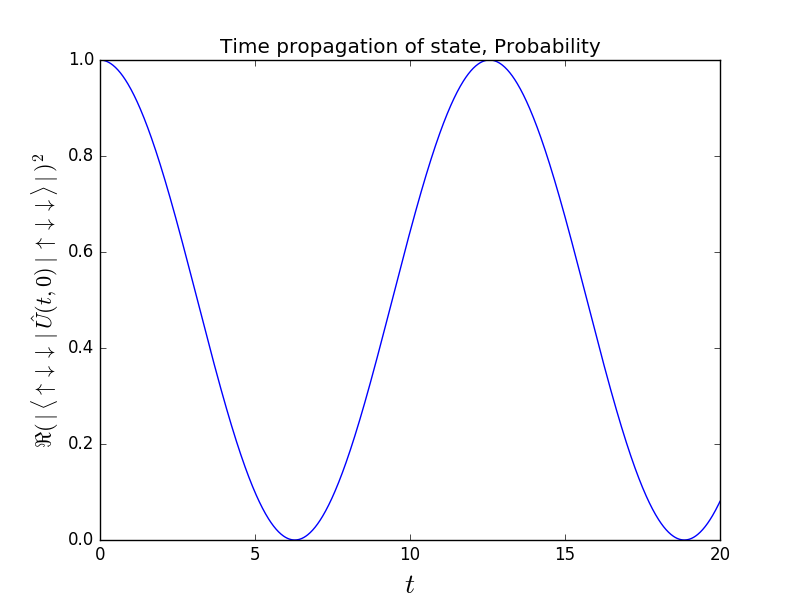
\includegraphics[width=0.9\textwidth]{figures/probability.png}
	\caption{Probability that state remains in initial state $\ket{\uparrow\downarrow\downarrow}$.}
	\label{fig:probability}
\end{figure}

An analytical expression for the probability will look something like this
\begin{equation*}
P(t) = \abs{\bra{\uparrow\downarrow\downarrow}\hat{U}(t,0)\ket{\uparrow\downarrow\downarrow}}^2
\end{equation*}
rewriting the expected value of this exuation as a sum of energy eigenvalue states
\begin{equation*}
\bra{\uparrow\downarrow\downarrow}\hat{U}(t,0)\ket{\uparrow\downarrow\downarrow} =
\sum_n \abs{C_n}^2e^{iE_n}t/\hbar
\end{equation*}
then the probability becomes
\begin{equation}
P(t) = \sum_n\sum_m\abs{C_n}^2\abs{C_m}^2e^{-i(E_n-E_m)t/\hbar}=\sum_nC_n^4+\sum_{n\neq m}C_n^2C_m^2\cos(E_n-E_m)t/\hbar
\end{equation}
by employing Euler's formula and only including the real parts, because a probability is not a complex number.

%% ------------------- Problem 2 ------------- %%
\section{}
Here we consider a operator $e^{-\hat{H}s}$, where $s$ is a real positive number with units of inverse energy and $\hat{H}$ is a know Hamiltonian. The ground state $\ket{E_0}$ is not known, but we do know a way to compute $\ket{\psi(s)}\equiv e^{-\hat{H}s}\ket{\psi}$ efficiently for any $s$ and $\ket{\psi}$. This can then be used to compute the ground state expected value  $\bra{E_0}\hat{O}\ket{E_0}$ for a given Hermitian operator $\hat{O}$.

First, let us assume that a state $\ket{\psi}$ can be written as a linear combination of eigenstates, such that
\begin{equation*}
\ket{\psi(s)}=e^{-\hat{H}s}\ket{\psi}=e^{-\hat{H}s}\sum_i C_i\ket{E_i}=\sum_i e^{-E_i s}C_i\ket{E_i}
\end{equation*}
if $s$ is sufficiently large, $s>>1$, all the terms in the sum above will be killed except for the ground state 
\begin{equation*}
\ket{\psi} \approx e^{-E_0s}C_0\ket{E_0}
\end{equation*}
Then we get
\begin{align}
\braket{\psi(s)} &= e^{-2E_0s}\abs{C_0}^2\braket{E_0}=e^{-2E_0s}\abs{C_0}^2 \label{eq:psis1} \\
\bra{\psi(s)}\hat{O}\ket{\psi(s)} &= e^{-2E_0s}\abs{C_0}^2\bra{E_0}\hat{O}\ket{E_0} \label{eq:psis2}
\end{align}
Dividing equation \ref{eq:psis2} by equation \ref{eq:psis1} will for a large $s$ yield the desired result
\begin{equation}
\lim_{s\to\infty}\frac{\bra{\psi(s)}\hat{O}\ket{\psi(s)}}{\braket{\psi(s)}}=\bra{E_0}\hat{O}\ket{E_0}
\end{equation}

An interesting matter to look into further is how big $s$ must be. If there is an energy difference of $dE$ between the lowest and second lowest state, then knowing the value of $dE$ allows one to quantify how big $s$ must be by employing the following expression
\begin{equation*}
\ket{\psi(s)}\approx e^{-E_0s}(C_0\ket{e_0}+e^{-sdE}C_1\ket{E_1}+\dots)
\end{equation*}

\pagebreak
\begin{appendix}
\section{Numerical computation of $H\ket{\uparrow\downarrow\downarrow}$}
\label{app:updndn}
\lstinputlisting[language=Python, lastline=51, showstringspaces=false]{scripts/tensors.py}

\pagebreak
\section{Calculation of $[H,S_{tot}]$}
\label{app:prob1.5}
\begin{figure}[ht]
	\centering
	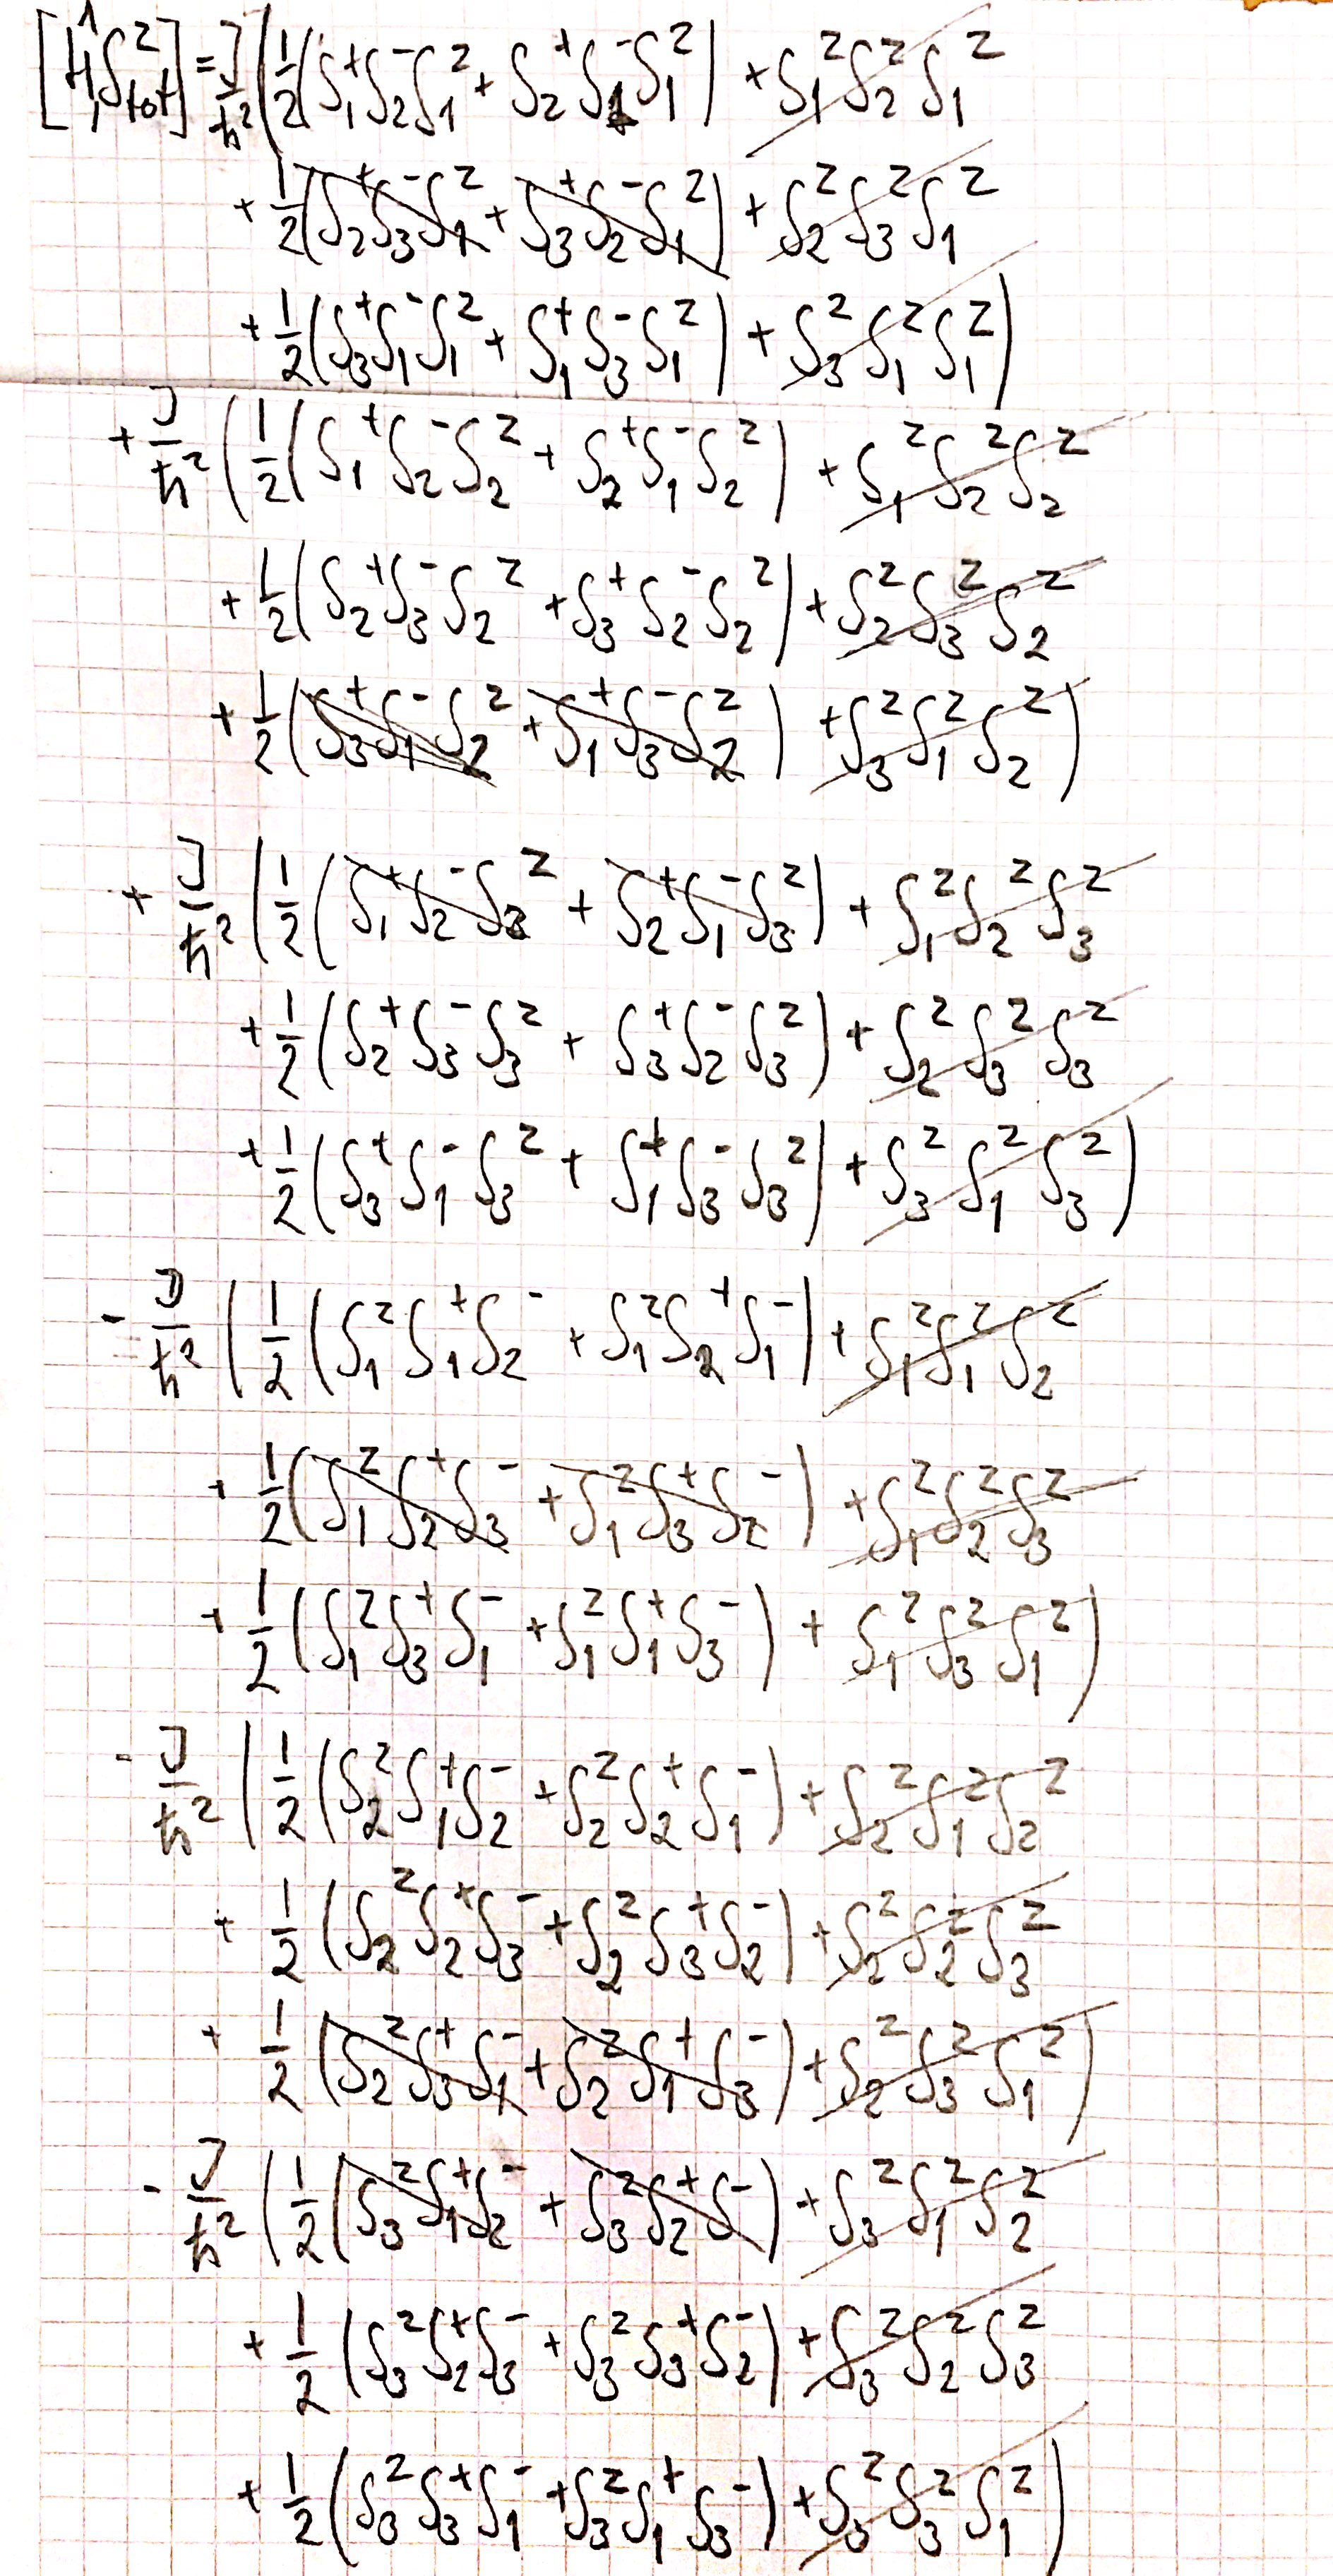
\includegraphics[width=0.58\textwidth]{figures/Problem1_5_1.jpg}
\end{figure}

\begin{figure}[ht]
	\centering
	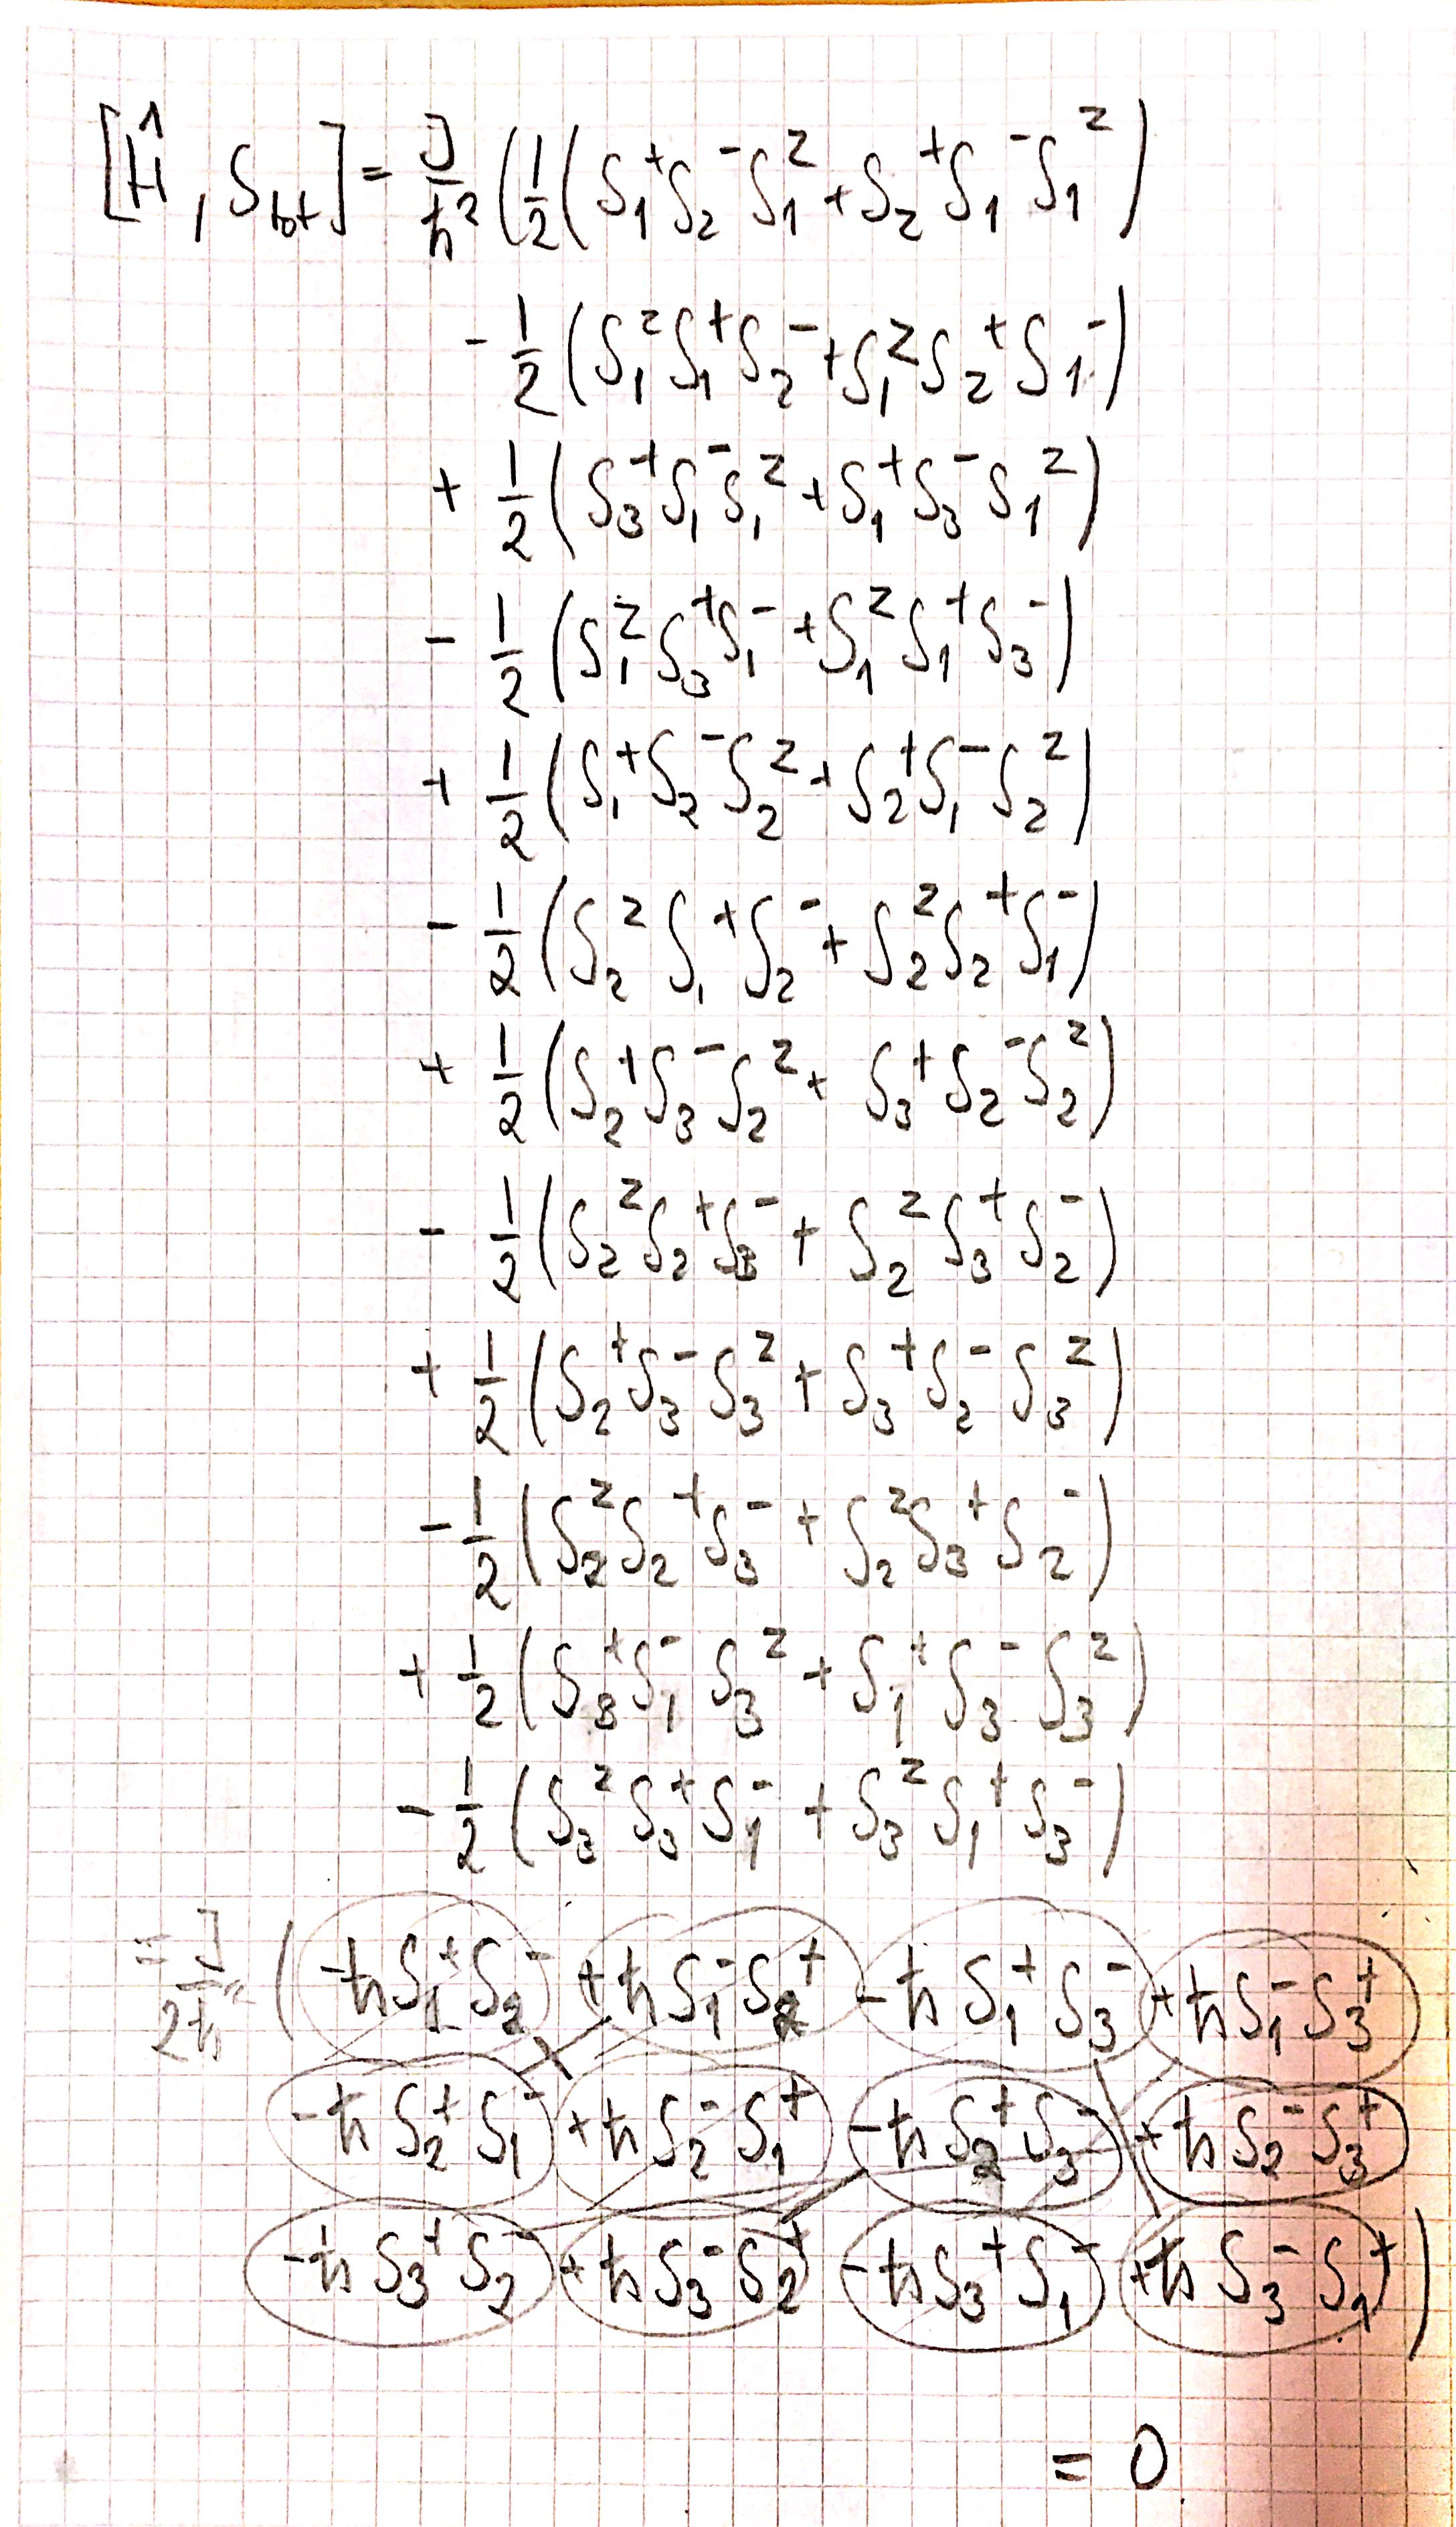
\includegraphics[width=0.75\textwidth]{figures/Problem1_5_2.jpg}
\end{figure}
\end{appendix}

\end{document}
